\section{Einführung}
Wird Licht von Objekten gestreut, deren Ausdehnung in der Größenordnung der Wellenlänge liegt, so lässt sich die Lichtausbreitung nicht mehr wie in der geometrischen Objekt durch Strahlen beschreiben. Stattdessen führt der Wellencharakter des Lichtes zu einer Beugung und es entstehen Interferenzmuster.

Das Prinzip von Huygens-Fresnel besagt, das jeder Punkt auf einer Wellenfront als Ausgangspunkt einer Kugelwelle gesehen werden kann. Zu einem späteren Zeitpunkt lässt sich die Ausbreitung der Welle berechnen, indem man diese Elementarwellen überlagert.

\subsection{Frauenhofer-/Fernfeldbeugung}
In der Fernfeldbeugung wird angenommen, dass die einfallenden und die aufallenden Wellen nahezu eben sind. Dies ist eine gute Näherung, wenn die Lichtquelle weit vom Beugungselement und dieses weit vom Schirm entfernt ist.
\subsubsection{Beugung am Spalt}
Für einen Spalt mit Breite $b$ ergibt sich in einem Winkel $\theta$ zur optischen Achse die Intensität 

\begin{equation}
I(\vartheta)\propto b^2\left\{\frac{sin\beta}{\beta}\right\}^2
\label{spaltintens}
\end{equation}
\begin{figure}[!htb]
  \centering
  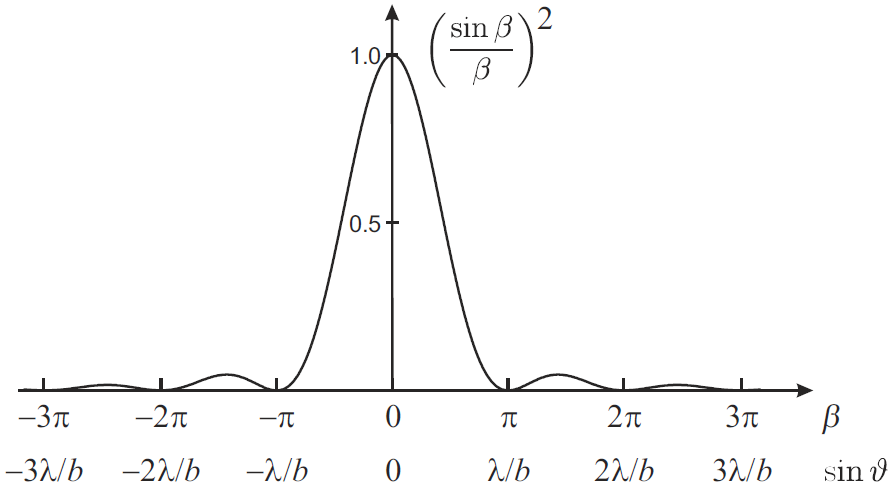
\includegraphics[width=.8\textwidth]{res/spaltintens}
  \caption{Lichtintensität hinter einem Beugungsspalt\footcite{anleitung-ss2015}}
  \label{fig:spaltintens}
\end{figure}
mit $\beta=(kb\sin\vartheta)/2=\pi\frac{b}{\lambda}\sin\vartheta$. Die Funktion $(\sin\beta/\beta)^2$ ist in \cref{fig:spaltintens} abgebildet. Sie hat für $\beta=0$ das Maximum 1 und Nullstellen für $\beta=\pm\pi, \pm 2\pi,\dots$. Auf einem in großem Abstand zum Spalt aufgestellten Schirm sind Minima zu sehen für Winkel $\vartheta$ mit 
\begin{equation}
\sin\vartheta=m\frac{\lambda}{b} \qquad\text{wobei}\qquad m=\pm1,\pm2,\dots
\label{spaltmin}
\end{equation}
\subsubsection{Beugung am Gitter}
Ein Gitter besteht aus abwechselnd lichtdurch- bzw. undurchlässigen Sektoren. Die Gitterkonstante $g$ ist der Abstand zwischen benachbarten Streifen, $b$ die Breite eines Streifens und $N$ die Anzahl der Gitterlücken. Die Intensität bei einem Winkel $\vartheta$ zur optischen Achse beträgt dann
\begin{equation}
I(\vartheta)\propto \left[\frac{\sin(N\gamma)}{\sin\gamma}\right]^2\cdot\left[\frac{\sin\beta}{\beta}\right]^2 \qquad\text{mit}\\
\gamma=\pi\frac{g}{\lambda}\sin\vartheta \qquad\text{und}\qquad\beta=\pi\frac{b}{\lambda}\sin\vartheta=\frac{b}{g}\gamma
\label{gitterintens}
\end{equation}
\begin{figure}[!htb]
  \centering
  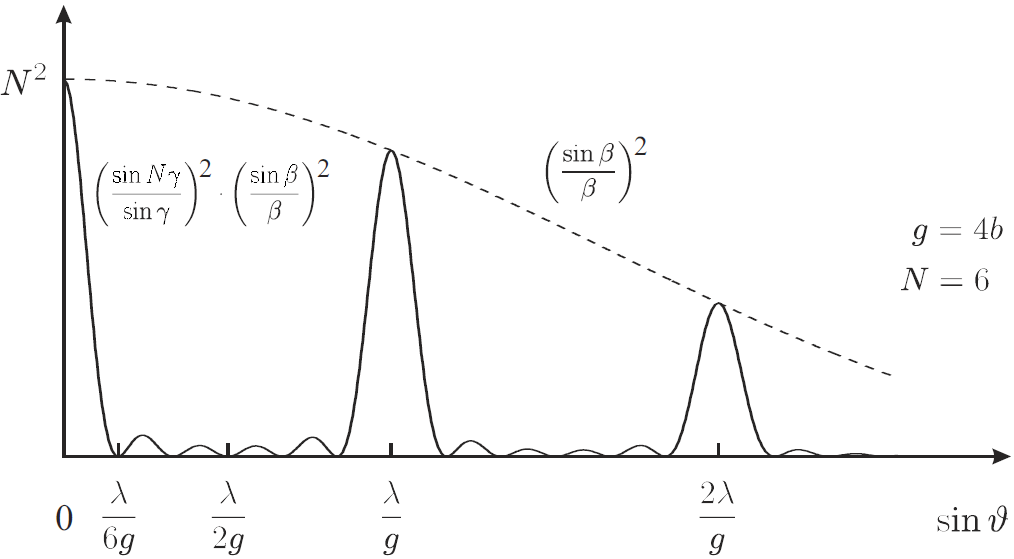
\includegraphics[width=.8\textwidth]{res/gitterintens}
  \caption{Lichtintensität hinter einem Gitter\footcite{anleitung-ss2015}}
  \label{fig:gitterintens}
\end{figure}
Die Maxima des Gitterfaktors $[\sin(N\gamma)/\sin\gamma]^2$ 
\begin{equation}
\sin\vartheta_m=m\frac{\lambda}{g} \qquad\text{mit}\qquad m=0,\pm1,\pm2,\dots
\label{gittermax}

entsprechen Hauptmaxima auf dem Schirm.

\section{Versuche}
\section{Diskussion}

